\title{Data Subsampling}

{{navbar}}

\subsubsection{Data Subsampling}

Running algorithms which require the full data set for each update
can be expensive when the data is large. In order to scale inferences,
we can do \emph{data subsampling}, i.e., update inference using
only a subsample of data at a time.

(Note that only certain algorithms support data subsampling such as
\texttt{MAP}, \texttt{KLqp}, and \texttt{SGLD}. Also, below we
illustrate data subsampling for hierarchical models; for models with
only global variables such as Bayesian neural networks, a simpler
solution exists: see the
\href{/tutorials/batch-training}{batch training tutorial}.)

\subsubsection{Subgraphs}

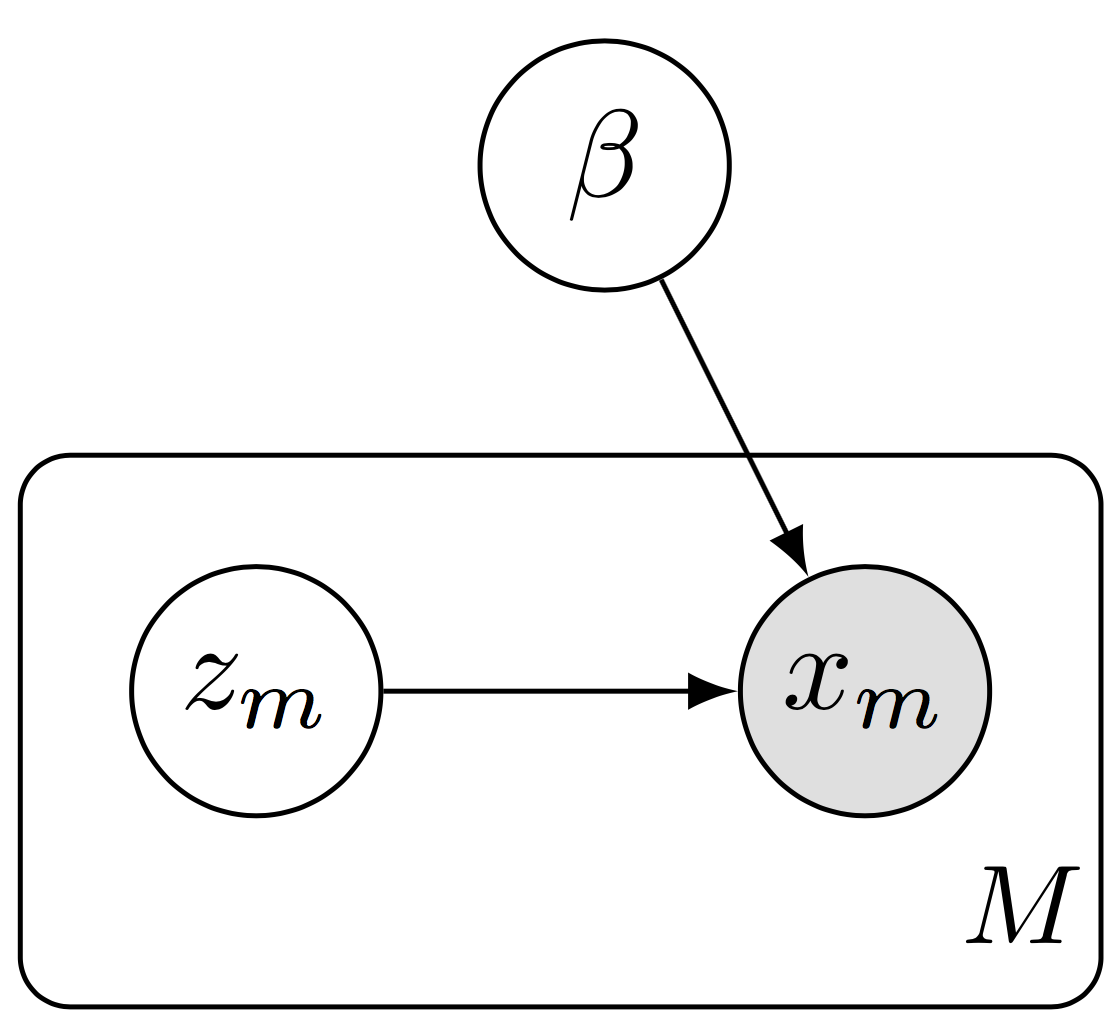
\includegraphics[width=250px]{/images/hierarchical_model_subgraph.png} \\
{\small\textit{Data subsampling with a hierarchical model. We define
a subgraph of the full model, forming a plate of size $M$ rather than
$N$.}}

In the subgraph setting, we do data subsampling while working with a
subgraph of the full model. This setting is necessary when the data
and model do not fit in memory.
It is scalable in that both the
algorithm's computational complexity (per iteration) and memory
complexity are independent of the data set size.

As illustration, consider a hierarchical model,
\begin{equation*}
p(\mathbf{x}, \mathbf{z}, \beta)
= p(\beta) \prod_{n=1}^N p(z_n \mid \beta) p(x_n \mid z_n, \beta),
\end{equation*}
where there are latent variables $z_n$ for
each data point $x_n$ (local variables) and latent variables $\beta$
which are shared across data points (global variables).

To avoid memory issues, we work on only a subgraph of the model,
\begin{equation*}
p(\mathbf{x}, \mathbf{z}, \beta)
= p(\beta) \prod_{m=1}^M p(z_m \mid \beta) p(x_m \mid z_m, \beta).
\end{equation*}
More concretely, we might define a mixture of Gaussians over
$D$-dimensional data $\{x_n\}\in\mathbb{R}^{N\times D}$. There are $K$
latent cluster means $\{\beta_k\}\in\mathbb{R}^{K\times D}$ and a
membership assignment $z_n\in\{0,\ldots,K-1\}$ for each data point
$x_n$.

\begin{lstlisting}[language=Python]
from edward.models import Categorical, Normal

N = 10000000  # data set size
M = 128  # minibatch size
D = 2  # data dimensionality
K = 5  # number of clusters

beta = Normal(loc=tf.zeros([K, D]), scale=tf.ones([K, D]))
z = Categorical(logits=tf.zeros([M, K]))
x = Normal(loc=tf.gather(beta, z), scale=tf.ones([M, D]))
\end{lstlisting}

For inference, the variational model follows the same factorization as
the posterior,
\begin{equation*}
q(\mathbf{z}, \beta) =
q(\beta; \lambda) \prod_{n=1}^N q(z_n \mid \beta; \gamma_n),
\end{equation*}
parameterized by $\{\lambda, \{\gamma_n\}\}$.
Again, we work on only a subgraph of the model,
\begin{equation*}
q(\mathbf{z}, \beta) =
q(\beta; \lambda) \prod_{m=1}^M q(z_m \mid \beta; \gamma_m).
\end{equation*}
parameterized by $\{\lambda, \{\gamma_m\}\}$. Importantly, only $M$
parameters are stored in memory for $\{\gamma_m\}$ rather than $N$.

\begin{lstlisting}[language=Python]
qbeta = Normal(loc=tf.Variable(tf.zeros([K, D])),
               scale=tf.nn.softplus(tf.Variable(tf.zeros[K, D])))
qz_variables = tf.Variable(tf.zeros([M, K]))
qz = Categorical(logits=qz_variables)
\end{lstlisting}

For illustration, we perform inference with \texttt{KLqp}, a variational method
that minimizes the divergence measure $\text{KL}(q\| p)$.

We instantiate two algorithms: a global inference over $\beta$ given
the subset of $\mathbf{z}$ and a local inference over the subset of
$\mathbf{z}$ given $\beta$.
We also pass in a TensorFlow placeholder \texttt{x_ph} for the data,
so we can change the data at each step. (Alternatively,
\href{/api/data}{batch tensors} can be used.)

\begin{lstlisting}[language=Python]
x_ph = tf.placeholder(tf.float32, [M])
inference_global = ed.KLqp({beta: qbeta}, data={x: x_ph, z: qz})
inference_local = ed.KLqp({z: qz}, data={x: x_ph, beta: qbeta})
\end{lstlisting}

We initialize the algorithms with the \texttt{scale} argument, so that
computation on \texttt{z} and \texttt{x} will be scaled appropriately.
This enables unbiased estimates for stochastic gradients.

\begin{lstlisting}[language=Python]
inference_global.initialize(scale={x: float(N) / M, z: float(N) / M})
inference_local.initialize(scale={x: float(N) / M, z: float(N) / M})
\end{lstlisting}

Conceptually, the scale argument represents scaling for each random
variable’s plate, as if we had seen that random variable $N/M$ as many
times.

We now run inference, assuming there is a \texttt{next_batch} function
which provides the next batch of data.

\begin{lstlisting}[language=Python]
qz_init = tf.initialize_variables([qz_variables])
for _ in range(1000):
  x_batch = next_batch(size=M)
  for _ in range(10):  # make local inferences
    inference_local.update(feed_dict={x_ph: x_batch})

  # update global parameters
  inference_global.update(feed_dict={x_ph: x_batch})
  # reinitialize the local factors
  qz_init.run()
\end{lstlisting}

After each iteration, we also reinitialize the parameters for
$q(\mathbf{z}\mid\beta)$; this is because we do inference on a new
set of local variational factors for each batch.

This demo readily applies to other inference algorithms such as
\texttt{SGLD} (stochastic gradient Langevin dynamics): simply
replace \texttt{qbeta} and \texttt{qz} with \texttt{Empirical} random
variables; then call \texttt{ed.SGLD} instead of \texttt{ed.KLqp}.

\subsubsection{Advanced settings}

If the parameters fit in memory, one can avoid having to reinitialize
local parameters or read/write from disk.  To do this, define the full
set of parameters and index them into the local posterior factors.

\begin{lstlisting}[language=Python]
qz_variables = tf.Variable(tf.zeros([N, K]))
idx_ph = tf.placeholder(tf.int32, [M])
qz = Categorical(logits=tf.gather(qz_variables, idx_ph))
\end{lstlisting}

We define an index placeholder \texttt{idx_ph}. It will be fed index
values at runtime to determine which parameters correspond to a given
data subsample.
As an example, see the script for
\href{https://github.com/blei-lab/edward/blob/master/examples/probabilistic_pca_subsampling.py}
{probabilistic principal components analysis} with stochastic
variational inference.

An alternative approach to reduce memory complexity is to use an
inference network \citep{dayan1995helmholtz}, also known as
amortized inference \citep{stuhlmuller2013learning}.  This can be
applied using a global parameterization of $q(\mathbf{z}, \beta)$.
For more details, see the
\href{/tutorials/inference-networks}{inference networks tutorial}.

In streaming data, or online inference, the size of the data $N$
may be unknown, or conceptually the size of the data may be
infinite and at any time in which we query parameters from the online
algorithm, the outputted parameters are from having processed as many
data points up to that time.
The approach of Bayesian filtering
\citep{doucet2000on,broderick2013streaming} can be applied in Edward using
recursive posterior inferences; the approach of population posteriors
\citep{mcinerney2015population} is readily applicable from the subgraph
setting.

In other settings, working on a subgraph of the model does not
apply, such as in time series models when we want to
preserve dependencies across time steps in our variational model.
Approaches in the literature can be applied in Edward
\citep{binder1997space,johnson2014stochastic,foti2014stochastic}.

\subsubsection{References}\label{references}
